Random forest là một phương pháp học kết hợp (ensemble) cho các bài toán phân lớp, hồi quy bằng việc xây dựng nhiều cây quyết định (Decision Tree) khi huấn luyện. Với bài toàn phân loại, đầu ra của Random forest là lớp tương ứng được lựa chọn bởi đa số các cây quyết định. Random forest giúp giảm nhẹ đặc tính overfit với tập huấn luyện ở Cây quyết định, vì vậy thường nó sẽ có độ chính xác cao hơn sử dụng mô hình Cây quyết định.

\begin{figure}[h!]
    \centering
    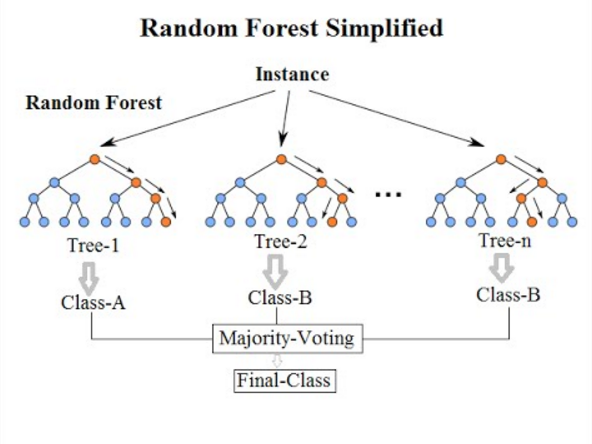
\includegraphics[width=0.6\textwidth]{figures/Random_forest_diagram_complete.png} % độ rộng ảnh bằng 0.6 độ rộng tối đa của một dòng
    \caption{Biểu đồ của một mô hình Random forest} % caption của ảnh
    \label{fig:2} % label của ảnh dùng để reference ảnh. Trong bài viết có chỗ nào cần nói "tại hình 1" thì viết "tại hình \ref{fig:1}"
\end{figure}

Random forest cho bài toán phân loại được xây dựng dựa trên các thành phần sau:
\subsubsection{Các cây quyết định:}
Cây quyết định là phương pháp phổ biến được sử dụng cho các bài toán học máy. 
Một cây quyết định là một cấu trúc dữ liệu với dạng giống như lưu đồ, với mỗi nút trong đại diện cho một kiểm thử trên một thuộc tính, mỗi nhánh đại diện cho kết quả của kiểm thử đó, và mỗi nút lá đại diện cho một lớp nhãn. Đường đi từ gốc tới lá biểu diễn một quy tắc phân loại.

Để xây dựng một cây quyết định, có nhiều thuật toán được sử dụng như $ID3, CART,\dots$. Tương ứng với mỗi thuật toán, sẽ có các chỉ số khác nhau được sử dụng để đánh giá. Ví dụ như thuật toán $ID3$ sử dụng chỉ số \emph{information gain}, thuật toán \emph{CART} sử dụng chỉ số \emph{Gini index}. Ở đây chúng em xin đề cập tới thuật toán \emph{CART} với chỉ số \emph{Gini index}:
Để tính Gini index, trước hết cần tính chỉ số Gini, chỉ số Gini tính ở từng nút như sau:
\begin{equation*}
    Gini = 1 = \sum^C_{i=1}(p_i)^2
\end{equation*}

Trong đó $C$ là số lớp cần phân loại, $p_i = n_i/N$, với $n_i$ là số lớp thứ $i$ và $N$ là số lượng phần tử ở nút đó, $N = \sum^N_{i=1}n_i \Rightarrow \sum^N_{i=1}p_i = 1$

Do $0 <= p_i <= 1 \forall i$ và $\sum^N_{i=1}p_i=1$ nên:
\begin{equation*}
    \sum^C_{i=1}(p_i)^2 <= (\sum^C_{i=1}p_i)^2 = 1 \Rightarrow Gini >= 0
\end{equation*}
\begin{equation*}
    \sum^C_{i=1}(p_i)^2 >= \frac{(\sum^C_{i=1}p_i)^2}{C} = 1/C \Rightarrow Gini <= (C-1)/C
\end{equation*}

Sau khi tính được Gini ở nút cha và $K$ nút con, ta tính được chỉ số Gini index:
\begin{equation*}
    GiniIndex = Gini(p) - \sum^K_{i=1}\frac{m_k}{M}Gini(c_k)
\end{equation*}

Trong đó $Gini(p)$ là chỉ số Gini ở nút cha, $K$ là số nút con được tách ra, $Gini(c_k)$ là chỉ số Gini ở nút con thứ $k$. $M$ là số phần tử ở nút $p$, $m_i$ là số phần tử ở nút con thứ $i$, $\sum^K_{i=1}m_i = M$

Vì khi tách mình muốn chỉ số \emph{Gini} ở các node con nhỏ, nên \emph{Gini index} mình mong muốn càng lớn càng tốt. Để tìm điều kiện tách, mình thử ở tất các thuộc tính, mỗi thuộc tính thử một số giá trị chia, rồi so sánh xem điều kiện nào chỉ số Gini Index giảm nhiều nhất thì sẽ chọn để chia.

Cây có số bậc càng cao thì càng có khả năng học được những khuôn mẫu bất quy tắc từ dữ liệu huấn luyện, hay nói cách khác, chúng \emph{overfit} đữ liệu huấn luyện. Random forest cho bài toán phân loại là phương pháp lấy biểu quyết của nhiều cây quyết định, huấn luyện theo những hướng khách nhau trên cùng một tập huấn luyện, với mục tiêu giảm \emph{variance},đồng nghĩa với đó là tăng một chút \emph{bias} và mất mát một lượng nhỏ năng lực diễn giải (\emph{interpretability}), nhưng đổi lại sẽ giúp tăng cường năng lực của mô hình cuối.
\subsubsection{Bagging:} Thuật toán huấn luyện cho Random forest sử dụng kỹ thuật \emph{boostrap aggregating}, hay còn gọi là \emph{bagging}. Với một tập huấn luyện cho trước $X = x_1,\dots,x_n$, và biến phản hồi $Y=y_1,\dots,y_n$, bagging lặp lại việc lựa chọn một mẫu ngẫu nhiên thay cho tập huấn luyện và huấn luyện các Cây cho các mẫu dữ liệu này:
      \begin{algorithm}[h!]
          \DontPrintSemicolon
          Với $b = 1,\dots,B:$
          \begin{itemize}
              \item 1. Lấy $n$ mẫu từ dữ liệu $X, Y$; gọi là $X_b, Y_b$
              \item 2. Huấn luyện một cây phân loại trên $X_b, Y_b$
          \end{itemize}
          \caption{Thuật toán Bagging}
          \label{alg:Bagging}
      \end{algorithm}
      Sau khi huấn luyện, các dự đoán cho dữ liệu chưa nhìn thấy $x'$ được xác định bằng cách biểu quyết (\emph{vote}) theo đa số.
\subsubsection{Feature Bagging:} 
      Ngoài ra, Random forest cũng có một phương pháp bagging khác gọi là \emph{feature bagging}, ý tưởng là tại mỗi bước chia ứng viên trong quá trình học, thuật toán sẽ chọn ra một tập con ngẫu nhiên các đặc trưng. Lí do là vì, nếu một nhóm đặc trưng (\emph{feature}) rất tốt trong việc dự đoán biến phản hồi, thì những feature này sẽ phải được lựa chọn nhiều lần trong các Cây. Ở một bài toán phân loại điển hình với $p$ đặc trưng, $\sqrt{p}$ các đặc trưng thường được sử dụng ở mỗi bước chia. 

